%%==================================================
%% demo.tex for BIT Thesis
%% modified by yang yating
%% version: 1.0
%% last update: Sep. 1st, 2017
%%==================================================

% 默认单面打印 oneside 、硕士论文模板 master

\documentclass[oneside, master]{BIT-thesis-grd}

% 打印选项: 双面打印 oneside;单面打印 twoside
% 模板选项: 硕士论文 master; 博士论文 doctor

\usepackage{hyperref}
%\usepackage[linesnumbered,boxed,commentsnumbered,ruled]{algorithm2e}
\usepackage[ruled,vlined]{algorithm2e}
\usepackage{caption}
\usepackage{subfigure}

\begin{document}

%%%%%%%%%%%%%%%%%%%%%%%%%%%%%%
%% 封面
%%%%%%%%%%%%%%%%%%%%%%%%%%%%%%

% 中文封面内容(关注内容而不是表现形式)
\classification{TQ028.1}
\UDC{540}

\title{基于深度学习的空指针引用缺陷检测系统的设计与实现}
\vtitle{基于深度学习的空指针引用缺陷检测系统的设计与实现}
\author{罗辉}
\institute{软件学院}
\advisor{田东海教授}
\chairman{计卫星教授}
\degree{工学硕士}
\major{软件工程}
\school{北京理工大学}
\defenddate{2018年5月}
%\studentnumber{**********}


% 英文封面内容(关注内容而不是表现形式)
\englishtitle{Design and implementation of null pointer reference defect detection system based on deep learning}
\englishauthor{Hui Luo}
\englishadvisor{Prof. Donghai Tian}
\englishchairman{Prof. **}
\englishschool{Beijing Insititute of Technology}
\englishinstitute{Software Institute}
\englishdegree{Master of Science}
\englishmajor{Software engineering}
\englishdate{June,2018}

% 封面绘制
\maketitle

% 中文信息
\makeInfo

% 英文信息
\makeEnglishInfo

%打印竖排论文题目
\makeVerticalTitle

% 论文原创性声明和使用授权
\makeDeclareOriginal

%%%%%%%%%%%%%%%%%%%%%%%%%%%%%%
%% 前置部分
%%%%%%%%%%%%%%%%%%%%%%%%%%%%%%
\frontmatter

% 摘要
%%==================================================
%% abstract.tex for BIT Master Thesis
%% modified by yang yating
%% version: 0.1
%% last update: Dec 25th, 2016
%%==================================================

\begin{abstract}
本文……。({\color{blue}{摘要是一篇具有独立性和完整性的短文,应概括而扼要地反映出本论文的主要内容。包括研究目的、研究方法、研究结果和结论等,特别要突出研究结果和结论。中文摘要力求语言精炼准确,硕士学位论文摘要建议500$\sim$800字,博士学位论文建议1000$\sim$1200字。摘要中不可出现参考文献、图、表、化学结构式、非公知公用的符号和术语。英文摘要与中文摘要的内容应一致。}})

\keywords{形状记忆;聚氨酯;织物;合成;应用 ({\color{blue}{一般选3~8个单词或专业术语,且中英文关键词必须对应。})}}
\end{abstract}

\begin{englishabstract}

   In order to exploit …….
   
\englishkeywords{shape memory properties; polyurethane;textile;synthesis;application}

\end{englishabstract}


% 加入目录
\tableofcontents

% 加入表格索引
%\listoftables

% 加入插图索引
%\listoffigures

%%%%%%%%%%%%%%%%%%%%%%%%%%%%%%
%% 正主体部分
%%%%%%%%%%%%%%%%%%%%%%%%%%%%%%
\mainmatter

%% 各章正文内容
%%==================================================
%% chapter01.tex for BIT Master Thesis
%% modified by yang yating
%% version: 0.1
%% last update: Dec 25th, 2016
%%==================================================
\chapter{绪论}
\label{chap:intro}
\section{本论文研究的目的和意义}

近年来,随着社会各方面的快速发展,移动互联和社交网络的普及,全球的数据量以指数级快速增长,人类社会已经迈入大数据时代\upcite{Lynch2008Big,Li2012Research,Wang2013Network}。随着计算机信息技术和多种新兴技术如云计算、物联网、分布式计算的快速发展,对大数据处理和挖掘成为可能,从浩瀚数据中挖掘出有用的知识,成为了学术界和工业界的研究的热点。

大数据是什么,麦肯锡全球研究所给出的定义是\upcite{McKinsey2011}:大数据一种数据集合,这种数据集合规模很大,在获取、存储、管理、分析等方面大大超出了传统数据库软件工具能力的范围,并且具有海量的数据规模、快速的数据流转、多样的数据类型和较低的价值密度四大特征。大数据数据量巨大,已经超出传统数据库的存储能力,目前,个人计算机硬盘容量可达TB量级,一些企业的数据量接近EB量级。大数据的处理速度快,因为数据量庞大,如何在海量数据中快速得到有用信息是十分重要的。大数据的种类繁多,数据可以被分为结构化数据和非结构化数据,结构化数据包括常见的关系数据库存储的数据类型,非结构化数据是数据结构不规则的数据,如网络日志数据、音频数据、视频数据、图片数据等等。非结构化数据的存在对数据的处理能力提出了更高的要求。大数据的数据量大,而价值密度却低。一般而言,价值密度和数据总量的大小成反比。所以,如何从海量的低价值的数据中挖掘出更有价值的信息,是一个重要的研究内容。另外,大数据还具有分布极其不规律,有用的信息隐藏程度很深等特点。从海量数据中,可以提炼出大知识,从而可以对人类社会带来很大的价值,这是大数据带来的机遇与挑战。

相比于传统数据的处理,大数据的计算模式主要分为两种,批量计算和流式计算。批量计算是将数据先存储下来,再对数据进行分批次的计算,这种方式对数据计算的实时性要求不高,主要适用于不需要及时处理数据的场景,但是其处理数据的精度和全面性有保证。现在常用的批处理计算系统主要有Apache的Hadoop框架\upcite{White2009Hadoop}。与之相反,流式计算不会先将数据存储起来,而是直接对数据进行计算,因此对数据的计算速度有很高的要求。流式计算一般直接对数据在内存中进行计算,实时性强,但对数据的处理的精确度要求较低。在流式计算中,只对数据进行一次读取,不存在再次读取情况,这是流式计算的“one-pass”原则。由此可见,批量计算和流式计算相互补充,为了达到更好的处理效果,一般场景下,可以将两种计算模式结合使用,结合两者的优势来处理数据。

现如今,数据呈爆炸式增长,流式数据的应用越来越广泛,流式计算的重要性越来越多地显示出来。数据的流式计算可以广泛地应用于生活和生产的多个方面,如金融市场,天气气象领域,航空航天领域,传感器网络和流量监控领域等等。流式数据是指按照时间顺序不断增加的动态数据序列,具有潜在的无限体积,其计算的实时性要求高,对精度的要求比较宽松\upcite{李圣2016大数据流式计算系统研究综述}。目前,主流的流式计算系统有Twitter的Storm,LinkedIn的Kafka\upcite{kafka2013, Auradkar2012Data},Yahoo的S4(Simple Scalable Streaming System)\upcite{Chauhan2012Performance, Xhafa2015Processing, Neumeyer2011S4},以及传统行业金融领域中比较知名的StreamBase\upcite{Patrizio2006StreamBase}和Borealis\upcite{Abadi2005The}等。

由以上可知,流式数据作为大数据的一种重要的形态,在多个领域中有着非常广泛的应用前景,但该技术作为近几年快速发展应用的技术,仍然具有很大的挑战,主要在数据的收集、存储、处理和可视化上面。流式数据的实时性和庞大的数据量,连续快速到达的特点,以及在线分析的应用需求,带来了挑战,也带来了很多机遇\upcite{孙玉芬2007流数据挖掘综述}。

\section{国内外研究现状及发展趋势}
%\label{sec:***} 可标注label
目前,随着各个领域中处理数据量的增大,流式计算模式的普遍应用,流式数据的处理越来越广泛,国内外很多大学和研究机构都对数据流的管理系统进行了研究,其中一种流式数据分析与处理的典型模型结构如图\ref{fig:fig1}所示\upcite{于戈2006数据流分析}。从中可以看出流式数据的处理系统模型在理论上主要包括两大类,一类是流式数据的预处理,一类是流式数据的数据挖掘。

流式数据分析与挖掘系统模型的数据来源是流式数据的采集器,传感器是一种常见的采集器,比如要获取发动机的数据,则使用发动机上的传感器进行采集。流式数据的预处理包括几部分,拿到原始数据后,可以根据实际处理需要,对原始数据进行汇总、压缩、降维或者动态索引等操作,得到一个概要的数据集或者是近似的数据集。数据的降维主要发生在数据维数较高的场景中,将高维的数据映射到低维的空间,其中,主成分分析(PCA)方法\upcite{croux2018robust}是一种广泛应用的高维数据的降维方法,该方法通过正交变换,将一组可能存在相关性的变量转换为一组线性不相关的变量,减少数据关系之间的重叠性,通过少数几个主成分来表示多个变量之间的内部结构,重新组合成一组新的互相无关的综合指标来代替原来的指标。数据的压缩可以减少数据的存储量,动态索引可以更快地查找数据。这些预处理操作可以降低时间复杂度和空间复杂度,可以去除原始数据中一些不必要的特征,减少数据中的噪音,对后续的数据处理具有很重要的意义。在数据的挖掘处理中,对数据进行统计分析,可以很好地体现数据的特征,如常见的平均值、方差、均值等特征值的统计;对数据进行趋势分析,可以根据历史数据的变化情况,对将要到来的数据进行预测,多用于金融财务和股价方面的预测;对数据进行频繁模式的挖掘,可以找出频繁地出现在数据集中的模式,比如项集、子序列或者子结构;对数据进行模式匹配,可以在浩瀚数据中找到特定的数据;对数据进行聚类分析和分类分析,可以将无分类的无规律的错综复杂的原始数据分为多类,每个类里的数据具有相似性,反映相同的规律性和特性;而对数据进行异常数据检测,可以找出不符合正常行为模式的数据,在网络入侵、金融欺诈和机器监测等方面具有重要应用。

\begin{figure}
	\centering
	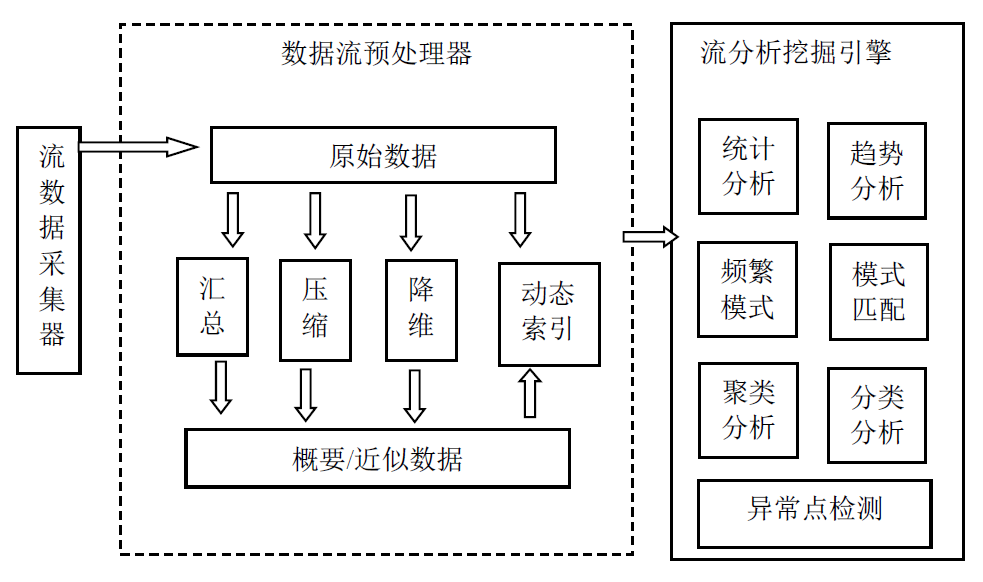
\includegraphics[width=0.75\textwidth]{figures/figure1x1}
	\caption{流式数据分析与挖掘系统模型}\label{fig:fig1}
\end{figure}

流式数据是连续的随着时间产生的数据序列,其中的数据可以是关系元组,也可以是数据项。目前在数据流研究领域存在多种数据流模型,分别有时序模型,现金登记模型和十字转门模型\upcite{孙玉芬2007流数据挖掘综述}。假设流式数据$X$的数据项为 ${x}_{1},{x}_{2},{x}_{3}, ..., {x}_{i}, ...$,数据项序列的下标$i$按顺序递增的,每个下标出现且只出现一次,则

\textbf{时序模型}:\ 每个数据项都代表所描述数据的属性值,$X[i] = {x}_{i}$。

\textbf{现金登记模型}:\ 多个数据项增量地描述数据的属性值,令${x}_{i} = \left(j,{I}_{i} \right)$,其中${I}_{i} > 0$,则有${X}_{i}[j] = {X}_{i-1}[j] + {I}_{i}$。

\textbf{十字转门模型}:\ 多个数据项描述数据的属性值,与现金登记模型的区别是现金登记模型的数据的属性值是一直在增大的,而十字转门模型的属性值可以增大,也可以减小。令${x}_{i} = \left(j,{U}_{i} \right)$,其中${U}_{i}$可以为正数,也可以为负数,则有${X}_{i}[j] = {X}_{i-1}[j] + {U}_{i}$。

其中,时序模型在流式数据的分析和挖掘中应用比较广泛。时序数据的数据项是一个关系元组$\left \langle t,s \right \rangle$,其中,$t$为时间戳,$s$为$t$时刻对应数据的属性值。数据流的数据具有时效性,因此数据携带有时间特征,通常为产生时刻的时间戳。流式数据要求对它进行实时性处理,数据项一旦流过就不复存在,不能再次进行访问,流式数据是源源不断产生的,具有潜在的无限体积,因此不能被全部存储下来。这些都是流式数据的特点。

\section{主要研究内容}
本文主要对流式数据的分析和处理进行研究。针对流式数据的特点,研究异常数据检测和数据压缩的常用算法,探讨在流式计算环境下,如何对算法更好地使用和优化加速,提高流式数据的处理效率。

异常数据检测的任务主要是从数据集中有效地检测出异常数据,异常数据是指在数据集中不符合正常行为模式定义的数据模式,也称为离散点。异常数据在数据集中所占比重小,采样困难,但是其中一般存在重要的信息,或者如果不进行检测,会对后续的处理产生重要的甚至灾难性的影响。比如在工业中,机器发生故障,此时通过异常点检测可以及时发现故障机器,减少生产损失。在日常生活中,电信欺诈和信用卡欺诈等行为已经造成了恶劣的社会影响,通过对正常数据生成模型,通过算法检测异常行为,可以有效地避免欺诈行为的发生,保护财产安全。异常数据检测还可以应用在网站维护方面,如果网站的访问量突然大幅度增加,可能原因是网站被黑客攻击或者被爬虫爬取数据等,所以异常数据的检测,在各个方面都具有实际的应用价值,对其进行研究具有重要的意义。目前为止形成了很多较为成熟且实用的方法,例如基于统计的方法、基于距离的方法和基于聚类的方法等。但是,由于时间复杂度和空间复杂度的影响,部分异常数据检测算法多为静态检测方法,适用于维度较低规模较小的数据集的离线检测,而流式数据大多维度高规模大,并且数据是源源不断到来的,数据量不断动态增长,行为模式可能随时间发生变化,所以在流式计算中,许多成熟的静态异常数据检测算法往往会出现检测结果发生偏差的问题,存在精度不高,运行效率低,不再适用等不足。

由大数据的特点可知,数据的数据量巨大,价值密度很低,对数据进行存储,不但需要耗费比较昂贵的存储资源,而且直接存储价值较低的原始数据没有意义。原始数据常常有噪音干扰,将原始数据直接存储后进行分析和挖掘会消耗大量的计算时间和存储空间,而且也会影响算法的准确性和可靠性。对原始数据进行压缩,可以减少数据的存储空间,节省存储资源,减少存储和后续的计算代价,而且数据压缩不计较细节上的差异,用整体数据的一些特征点来刻画整个数据的主要形态,保留这些主体特征,反应了数据的自身特点。数据压缩可以通过控制压缩度来实现不同的精度层次上的搜索和匹配,更能符合大多数领域只关心数据的变化规律或模式的需求。因此,数据压缩是数据预处理环节中重要的一项内容,具有重要的研究意义。在流式计算中,数据流是源源不断持续增长的,在对数据进行压缩时,数据产生的速度很快,如果压缩花费的时间较多,数据的处理不及时,未处理的数据容易拥塞聚集,最后很可能造成数据丢失的严重后果,因此在流式计算中,对压缩算法进行加速有很重要的意义。

本文主要研究流式数据的数据压缩和异常数据检测的时效性问题,来满足流式数据数据规模大,实时性强的特征,以及在线处理的要求。具体来说,针对流式数据的压缩与异常数据检测,完成以下工作:

第一,针对增量LOF算法在流式数据处理中存在的问题,提出了一种改进的增量LOF快速异常数据检测方法,该方法将数据的分布空间进行划分,将数据点映射到对应的网格单元中,可以有效解决流式数据数据量巨大无法在内存中存储计算的问题,而且减少了计算量。在此基础上,将同一网格内的数据点集中到中心一点,对数据点进行基于密度的异常数据检测,这种方法一方面可以减少数据的存储量,另一方面减少了需要进行距离运算的对象,大大减少了计算量,具有很好的时效性和较少的空间消耗。

第二,根据流式数据在线压缩的要求,采用滑动窗口算法与分段多项式拟合算法来对数据进行压缩。针对时序数据的采样时间是否是周期的,分析在多项式拟合中计算多项式系数时所用的最小二乘法的过程,分别采用缓存方法和增量计算的方法,减少计算量,来对数据压缩进行加速。

第三,通过实验,验证了本文针对数据压缩和异常数据检测提出的加速算法的有效性,减少了计算时间,保证了流式数据处理的高实时性。针对基于LOF方法的快速异常检测算法,通过实验对比,验证了本文的算法可以很好地适用于流式计算环境中,并且取得较好的结果,并且处理数据的速度更快,运行内存更小。针对数据压缩的加速   算法,通过实验,验证了本文提出的算法在不同多项式次数和不同误差率的情况下,可以很好地减少运行时间。

\section{章节安排}
本文主要分析异常数据检测和数据压缩在流式环境下的主流算法,探求算法的可行性和效率,基于这些算法提出改进,使计算提高效率,减少计算时间,达到加速效果。然后进行实验分析,保证其在实际中可以应用的可行性。本文的章节安排如下。

第一章,绪论,介绍了研究背景和意义,介绍了大数据的定义与特点,并介绍了大数据的计算模式,分为批量计算和流式计算,介绍了流式数据的特点和流式数据的处理计算模型。

第二章,针对异常数据检测方法和数据压缩方法,分别阐述了其应用背景,方法概述,和相关实现方法。这部分主要介绍异常数据检测方法和数据压缩方法的研究现状和主要使用算法。总结了异常数据检测的相关研究成果,介绍了主流的异常数据检测算法,包括基于统计的、基于聚类的、基于距离的和基于密度的方法。并且介绍了经典的算法,如iForest算法,LOF算法等等。总结了经典的数据压缩的方法,包括奇异值分解法、分段线性法、符号表示法和频域法,分析了各种方法优缺点及应用范围。以及很多方法都是应用在静态数据集中的,在流式数据的计算中,该如何改进使用这些方法。

第三章,介绍了异常数据检测方法的LOF方法和适用于流式数据的增量LOF算法,并且基于这两种方法,提出了一种新方法,该方法相比于增量的LOF方法,减少了存储量和计算量,更适合流式数据。

第四章,介绍了分段多项式压缩的方法,首先分析了在静态数据集上如何进行加速计算,然后针对流式数据给出了滑动窗口算法与分段多项式相结合的压缩算法,最后通过分析其压缩过程,对于不同的数据类型,给出了不同的加速计算方法。

第五章,实验章节,主要分为异常数据检测的对比实验和压缩算法的对比实验。异常数据检测算法主要与增量的LOF算法进行对比,压缩算法与原计算方法进行不同多项式次数的时间对比与不同分段方法的时间对比。

最后对论文的主要研究内容进行了总结。
\chapter{相关工作}
\label{chap:intro}

为了保证软件的可靠性和稳定性,在大量研究人员长期不懈地努力下,出现了很多针对软件缺陷的检测方法。这些方法可以在软件开发周期的不同阶段介入,检测的效率和效果也大不相同,最终涌现出了一批相对成熟的代码缺陷检测方法和工具。另一方面,随着软件数量的日益庞大,以及数据挖掘技术在各个研究领域的广泛应用,利用机器学习的方式来解决软件安全问题也逐渐成为了研究热点。

\section{程序静态分析技术}

静态分析技术即是在不运行程序,不依赖程序输入的情况下对程序代码进行分析的一项技术。这种技术有助于开发人员对代码结构的理解,同时也能检测潜在的安全缺陷(如SQL注入),运行时错误(如空指针引用缺陷)以及部分代码逻辑错误。它一般需要配合利用自动化工具执行分析。采用的技术有数据流分析,机器学习,语义精简等。可检测死锁,空指针,资源泄露,缓存区溢出,安全漏洞,竞态条件等软件缺陷,具有快速,准确,伸缩性强等特点。能够在代码开发阶段找到并修复多种问题,从而节省大量人力成本和时间。下面对部分静态分析方法涉及的相关技术进行简要的介绍。

符号执行\cite{king1976symbolic}是静态分析中较常用到的一种技术,它可以利用抽象符号描述程序执行过程中的变量值。这种方法可以很好地模拟程序的运行过程。相对于传统方法无法确定程序真实执行下各变量值的情况,此方法在对程序进行路径敏感分析时十分有效。不过因为符号执行方法会追踪程序中所有变量的所有取值空间,所以在应用于大规模代码进行分析时,可能会导致分析的可能路径数量迅速增多,因此在应用该方法的时候,往往会采取优化路径数量的方法即选择部分可能性最高的路径进行分析,这样虽然可以避免状态爆炸的产生,但是也难免会导致分析精度的下降。

PREfix\cite{bush2000static}是一种针对C语言的静态分析工具,它采用了符号执行的方法。该工具可以对程序每个可能的执行过程进行抽象建模,静态地模拟程序的多个可能执行路径,同时利用约束求解对程序分析过程中出现的约束集合进行检查。此工具能够做到路径敏感的缺陷检查,但是由于符号执行方法的特性,为了避免状态爆炸的情况出现,它只能选取部分路径进行分析,这就导致了分析精度的不理想。

模型检查\cite{jhala2009software}也是一种常见的静态分析技术,通常的做法是构建有限状态机或者有向图等抽象模型,再对构造出的模型进行遍历来检验待检测系统的部分性质。SLAM\cite{ball2001automatically}是一种具有代表性的基于模型检查的静态分析工具。它可以从待检测代码中抽象出一个布尔程序并加以验证。在得到的错误报告中逐个检查,找出所有误报,进而根据这些误报对抽象的布尔程序进行调优,经过不断迭代,最终可以取得很好的效果。

同样是应用于程序验证的技术,不同于模型检查,定理证明\cite{tiwari2007logical}是基于语义的程序分析方法。但是由于采用了消解原理的定理证明器,而这种方法对整数域和有理数域相关的运算不是很好处理,所以应用在程序分析领域显得不是特别合适。基于这种问题,研究人员通常会选择各种判定过程来确定公式是否是定理。ESC\cite{flanagan2013pldi}就是一个采用了定理证明技术的半自动化工具,它在分析程序的过程中需要外界指定所涉及的类不变量,过程不变量以及循环不变量。

除了上面提到的3种技术,抽象解释\cite{cousot1977abstract}的应用更加广泛,它是数据流分析的理论基础。1977年P.Cousot和R.Cousot
共同提出了抽象解释的理论,应用该理论分析程序时就不需要拘泥于程序最底层的具体细节上可以在更高的角度上去观察和思考。传统解释器可以知道程序中每个变量具体的值从而得到具体值域,而抽象解释不同与传统解释的地方就是可以得到一个更高阶的抽象值域。如果将一个传统解释器迁移到抽象解释器,几乎等同于构造一个函数把具体值域映射到抽象值域。如图\ref{fig:figure2-1}所示,我们可以将无限的整数具体值域抽象成正,负,零三个抽象值域,这个过程只需要实现一个抽象函数$\alpha$即可完成。
 \begin{figure}
	\centering
	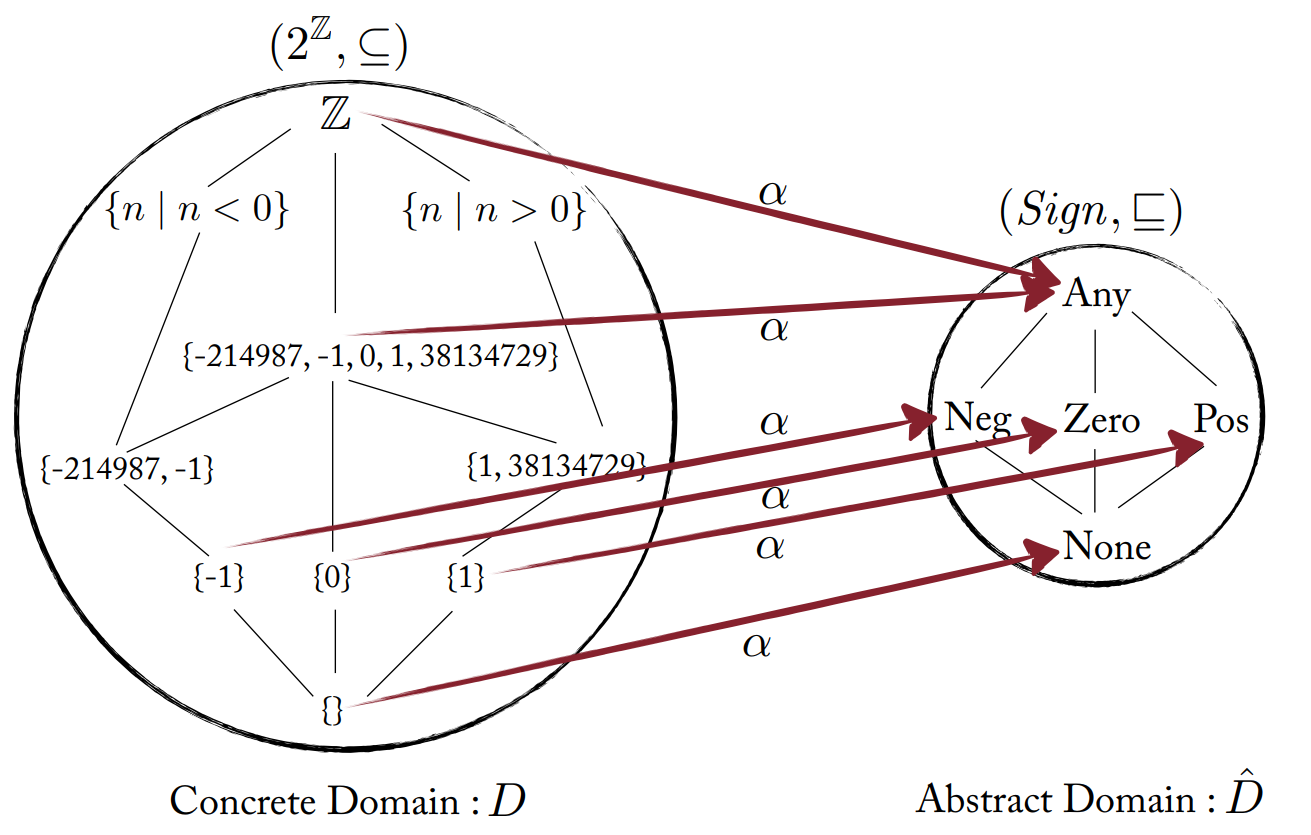
\includegraphics[width=0.70\textwidth]{figures/AbstractInterpretation2-1}
	\caption{将整数空间的具体值域映射到抽象值域}\label{fig:figure2-1}
\end{figure}

抽象解释理论实际上是从代码中抽象出一些能够刻画我们想要分析的问题所需要的特征,本质上还是为了提升分析的效率而损失部分分析精度的方法。但是如果应用得当,还是可以获得很大的收益,现在几乎所有的数据流分析方法都应用了该理论。

总的来说,静态分析技术在不运行代码的情况下进行分析有效避免了程序运行环境的苛刻要求,可以针对程序的规模采取灵活的分析方法,从而具备了较早发现缺陷,较低的分析成本,较高的覆盖率和自动化程序等优点。但是由于往往需要对分析精度进行部分舍弃,导致了分析结果的漏报率和误报率都无法达到特别理想的水平。

\section{静态分析技术在空指针引用缺陷检测的应用}
针对空指针引用缺陷,研究人员已经利用静态分析技术做出了很多实践并取得了一定成果。

研究人员利用静态分析技术在Java空指针引用缺陷上进行了大量的工作,产生了很多检测空指针引用的工具和技术,这些技术可粗略的分为指针引用验证\cite{madhavan2011null}和空指针引用\cite{xie2007saturn}缺陷检测两大类。前者侧重于如何验证程序中的指针是否为空。后者侧重于如何尽可能多的发现程序中的空指针引用。指针引用验证技术是基于需求驱动的思想\cite{wang2015},一般是首先识别出指针,再沿着控制流后向的验证指针是否为空。空指针引用缺陷检测一般是在进行数据流分析\cite{wangxu2015}、指针分析的基础上,根据一些规则基于控制流前向的检测。两者通常都需要进行数据流分析与指针分析。

Salsa\cite{loginov2008verifying}是一个致力于验证Java代码中指针引用安全性验证的工具,通过定制的数据表示形式进行前向数据流分析,通过对传播深度和数据流传播路径数量的简单限制来获得方法的可扩展性,同时依赖预先进行的必然别名分析来提高方法间数据流分析的准确性。由于一些空指针的引用需要经过多层方法调用链才有可能触发,这种验证方式会产生很多漏报的同时,效率也不理想。数据流分析技术具有十分灵活的特点,为了提高效率,Ravichandhran Madhavan\cite{madhavan2011null}等提出了一种过近似的最弱前置条件分析方法以验证Java程序中指针的安全性,该方法通过需求驱动的前向数据流分析大幅提升了单个引用的分析效率,该方法试图找到程序入口处可能满足被分析程序点的引用不安全的条件,如果存在这样的条件,则可以判定该引用不安全。此方法的数据流事实为有限的谓词集合,通过有选择地限制谓词集合的大小以及传播路径的数量,该方法可以做到低延迟的流敏感,上下文敏感的sound分析,利用Wala\cite{wala}程序分析框架,可以取得较好的验证引用安全的效果,但是过于追求针对单个引用的需求驱动分析,在对大规模代码中的引用进行批量分析时性能欠佳。

空指针检测相比于指针安全性验证更加具有实用性,而误报率和漏报率是检验工具实用性的重要指标,空指针检测工具大多不追求完美的正确率,而将较低的误报率和较高的召回率作为最重要的目标。

检测工具Xylem\cite{nanda2009accurate}从每一个指针引用出发,进行基于需求驱动的后向数据流分析,并将谓词作为数据流事实,目标是能够高效的检测出最重要的空指针引用,在进行分析时采取的是不完全可靠的分析方法,检测结果存在较多漏报。

北京邮电大学的杨睿\cite{yangrui2012}提出一种Java中空指针引用故障的静态检测方法,将空指针引用问题抽象为一类故障模型,并以故障模式状态机来形式化描述此类故障模型,然后根据故障状态机的创建条件及待检测代码的语义信息确定是否创建该类型的状态机,并将创建的状态机示例置于控制流图入口,根据数据流分析的结果对故障状态进行迭代以检测空指针引用问题。

中国矿业大学的姜淑娟\cite{jiang2017}提出一种空指针异常自动定位方法,该方法结合程序的静态分析技术,利用程序运行时的堆栈信息指导程序切片,然后对得到的切片进行空指针分析及别名分析,得出引发空指针异常的可疑语句集合,最终给出错误定位报告。

总体来看,以上这些分析方法都有各自的优缺点,但是目前无法找到一种完美的静态检测方法可以兼顾缺陷检测的误报率和漏报率。这也正是静态代码分析的短板,不仅是将复杂的缺陷解释出来很困难,对于结果的高误报率,往往显得无能为力。

\section{代码缺陷检测工具介绍}
对于空指针引用缺陷,工业界已经产生了很多优秀的检测工具,这些工具具有不同的实现原理,对空指针引用缺陷的检测结果也不尽相同。

FindBugs\cite{hovemeyer2005evaluating}\cite{hovemeyer2007finding}是一个开源的针对Java代码的缺陷静态检测工具,通过分析class文件,在字节码层级进行简单的前向数据流分析,对程序中的每一个引用的是否为null值的不同情况,给定相应的标识从而在触发可能的空指针调用时给出不同的告警等级。对于指针引用FindBugs总结出了一些经验规则,对不可达路径、控制流汇合、指针赋值语句、断言等特定情况定制了专用的检测规则,在进行过程间分析时,其主要依赖特定故障模式以及用户编码时给出的注解来推断空指针是否可能发生,所以它只能在特定场景下检测出空指针引用缺陷。

Jlint同样是一个开源静态代码检测工具,它通过执行数据流分析和构建锁图来查找缺陷,语义矛盾和同步问题。Jlint有两个独立的程序来执行语法和语义验证。通过使用手写扫描器和简单的自顶向下解析器,Jlint能够检测到一些代码缺陷,例如可疑地使用操作符优先级,没有切换代码中断,对构造体错误的假设等。同时,Jlint执行本地和全局数据流分析,计算局部变量的可能值并捕获冗余和可疑计算。通过执行全局方法调用分析,Jlint能够检测具有可能为“null”的形参的方法的调用,并且在没有验证“null”的方法中使用该参数。 Jlint还为类依赖项构建了锁依赖关系图,并使用该图来检测在多线程程序执行期间可能导致死锁的情况。除了死锁之外,当不同的线程可以同时访问相同的变量时,Jlint能够检测到可能的竞争条件问题。Jlint最大的特点就是检测的效率很高,但是由于使用的数据流分析十分有限,因此误报率也较高。

Infer是Facebook的开发团队在代码提交内部评审时,用来执行增量分析的一款静态分析工具,在代码提交到代码库或者部署到用户的设备之前找出缺陷。由OCaml语言编写的Infer目前能检测出空指针访问、资源泄露以及内存泄露,可对C、Java或Objective-C代码进行检测。Facebook使用Infer自动验证iOS和安卓上的移动应用的代码,bug报告的正确率达80\%。Infer通过捕获编译命令,把要被编译的文件转换为可用于分析潜在错误的中间语言格式。整个过程是增量进行的,意味着通常只有那些有修改过并提交编译的文件才会被Infer分析。Infer还集成了大量的构建或编译工具,包括Gradle、Maven、Buck、Xcodebuild、clang、make和javac。此外,Infer根植于两大基本理论之上,其一是霍尔逻辑,一种用于推理计算机程序正确性的形式系统,另一个是抽象解释,该理论用于测度程序语义的逼近结果,此外还涉及其它一些研究成果,例如Separation Logic和Bi-abduction。

Fortify SCA是一款应用广泛的商业工具,由知名的惠普公司出品 ,是一个白盒的、静态的软件源代码安全检测工具。它通过内部的五种主要分析引擎:语义、结构、控制流、数据流、配置流等对应用程序的源码进行静态分析,在分析的同时与该工具特有的软件安全漏洞规则集进行全面地查找、匹配,进而找出源代码中存在的各种缺陷和漏洞,并整理和产出缺陷报告。Fortify应用十分广泛,在世界范围内被大量公司用作内部源代码的质量安全检测工具。

Coverity是美国Coverity公司提供的可配置的用于检测软件缺陷和安全隐患的静态源代码分析解决方案,该工具基于布尔可满足验证技术应用于源代码分析引擎,分析引擎利用其专利的软件DNA图谱技术和meta-compilation技术,综合分析源代码、编译构建系统和操作系统等可能使软件产生的缺陷。Coverity是第一个能够快速、准确分析当今的大规模、高复杂度代码的工具,它解决了影响源代码分析有效性的很多关键问题,如编译兼容性,构建集成,高误报率,有效的错误根源分析等。

\section{深度学习技术在软件安全领域的应用}
深度学习是人工神经网络中一种多层级学习框架,试图通过构建深层网络模拟人脑感知抽象概念的能力。近年来,深度学习凭借着强大的特征学习能力,问题表达能力,数据容纳能力,掀起了又一次机器学习的浪潮,并在计算机视觉,语音处理,自然语言处理等众多领域取得了巨大进展,受到从学术界到工业界的广泛关注。现在,深度学习技术也开始渗透进软件工程的多个领域。

由于代码作为输入数据的特殊性以及复杂性,深度学习在软件安全方面常见的应用方法有两种。一种是以自然语言处理的思想来挖掘代码里的潜在信息;一种是将代码抽象为控制流图,以控制流图作为输入,压缩控制流图为向量之后进行分类回归运算。

Martin White\cite{white2016deep}等人提出了一种自然语言处理算法检测代码克隆的方法,该方法使用了两个RNN(递归神经网络)模型。先运用语法分析对代码进行预处理,然后用第一个RNN网络得到中间向量,再对代码进行词法分析得到代码的抽象语法树,将中间变量和语法树作为第二个RNN网络的输入,得到最终的检测结果。这种方法考虑到了代码文本上的相似性,忽视了代码结构上的相似性。

Hanjun Dai\cite{dai2016discriminative}提出了一种基于神经网络的图特征抽取的算法,能够根据不同的分类标准将代码控制流图压缩为多维的向量。Xiaojun Xu\cite{DBLP:journals/corr/abs-1708-06525}改进了该网络,通过将两段代码的控制流图成对的进行训练,从而检测两个二进制代码的相似度。通过该网络可以预测待测代码与已知缺陷代码的相似度,从而判断该代码是否为缺陷代码,为神经网络在检测代码缺陷方面的应用提供了新的思路。

\section{本章小结}
本章首先介绍了静态分析涉及的相关技术背景,然后以空指针引用的检测为例,介绍了国内外研究人员利用静态分析技术在空指针引用缺陷检测方面的进展,随后对一些业界成熟的静态代码缺陷检测工具,如Findbugs,Jlint,Infer,Fortify等进行了简要的介绍,最后对当下热门的深度学习技术在软件安全领域的应用进行了讨论。
%\chapter{总体架构}
本论文的目标是引入深度学习的方法针依据不同工具对代码的检测能力对大量缺陷代码进行分类,在使用多种检测工具对同一份代码进行检测时,可以有效得知这些工具针对这份代码的检测能力,然后利用这些工具的检测报告给出更精准的评判,从而提升检测精度。
\section{设计背景}
随着软件规模的增大,缺陷检测的难度和所需要的代价都越来越大,就Java语言的空指针引用异常的检测来说,目前业界存在着很多工具。如Findbugs,Jlint,Infer,Fortify等。他们在检测缺陷时使用了模式匹配,数据流分析,类型系统,模型检查等技术,由于不同的技术出于对检测精度和效率的权衡,他们所产出的检测报告往往各不相同,并且几乎都包含了大量的误报和漏报,开发人员在面对这样复杂的报告时,很难判断某条报告的准确性。NickRutar[A comparison of Bug Finding Tools for Java]等人针对五种Java语言的缺陷检测工具做了比较,发现没有任何一个单一的工具是完美的,此外,不同工具所产出的报告之间也有不小的差异。

基于这种情况,可以设想将多种工具的报告汇总到一起进行交叉验证,如果多个工具同时给出了同一个位置出现同一种缺陷的报告,我们有理由相信这个缺陷是真实可信的。因此,我们基于sonarqube平台开发了插件BIT-Detector,这个插件集成了Findbugs,Jlint,Infer和Fortify的能力,针对同一份待测代码,首先使用4种工具分别检测并给出报告,然后过滤出空指针引用缺陷,最后将4份报告的内容格式统一化从而进行比对,将不同工具同时检出的空指针引用缺陷作为BIT-Detector的输出,这样的结果理论上可以达到很高的准确率。

由于难以找到合适的空指针引用缺陷数据集,为了对这些工具进行合理的评测,本文采用一种创新的方式构建了一批可信的测试用例,这些用例的构造方法会在后面的章节详细说明。利用构建出来的7429个测试用例,我们针对上文提到的四种工具以及BIT-Detector进行了测试。图\ref{fig:figure3-1}反映了各个工具检出的空指针引用缺陷的重叠情况,表\ref{tab:table3-1}给出了不同工具检测的精度信息,同时还给出了BIT-Detector的数据。通过对比不难发现,各个工具的检测结果确实有较大差异,即使我们使用检测准确度最高的Findbugs,也会面临超过三分之一的误报,这些误报掺杂在检测报告中会给开发人员的缺陷修复带来很多困扰,可能很多时间和精力都会被浪费在验证缺陷的真实性上面。而保证报告的准确性应该是对检测工具的基本要求,即使不谈准确率,过多的漏报也会让人沮丧。显然,目前被广泛使用的各种检测工具还有很大的提升空间。

在检测过程中,我们也注意到选取所有工具共同检测缺陷作为输出结果的BIT-Detector在检测结果的准确率方面有着突出表现,相对于表现最好的Findbugs和Fortify,BIT-Detector有着22\%的准确率提升,而相对于准确率较低的Jlint而言,BIT-Detector的准确率提升则是成倍的增加。即使召回率的表现不尽人意,但是如果我们不将除了四种工具同时检测的缺陷排除在外,而是将四种工具的检测结果按照优先级排序,召回率在某种程度上来讲反而是提升的,如果按照这种方式处理检测报告,此时BIT-Detector的检测结果将自然地排在最前面,但是对其他结果的排序就成了一个棘手的问题,假如我们有四种工具,分别记为$T_{a}$,$T_{b}$,$T_{c}$,$T_{d}$。如果工具$T$在被测代码的$L$位置成功检出了某个缺陷$D$,则记为$E(T,L,D)=1$,反之则记为$E(T,L,D)=-1$。给定位置$L_{i}$,存在如下这种情况

\begin{equation}  
	\left\{  
	\begin{array}{lr}  
	E(T_{a},L_{i},D)=1, &  \\  
	E(T_{b},L_{i},D)=1, &  \\  
	E(T_{c},L_{i},D)=-1, &  \\  
	E(T_{d},L_{i},D)=-1, &  \\  
	\end{array}  
	\right.  
\end{equation} 

在这种情况下,开发人员很难判断位置$L_i$处是否存在缺陷$D$,如果我们知道工具



\begin{figure}
	\centering
	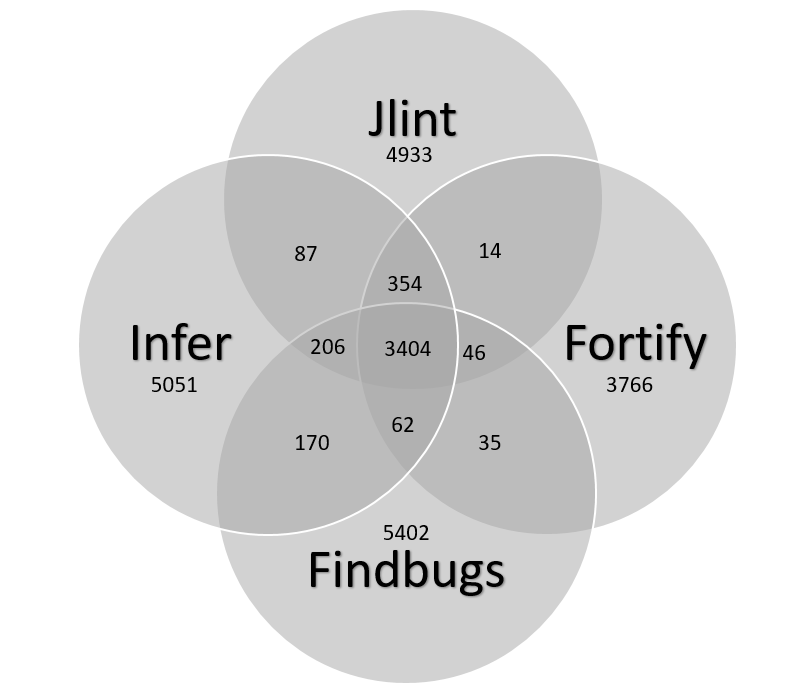
\includegraphics[width=0.70\textwidth]{figures/vnfigure3-1}
	\caption{4种工具在7429个测试用例上的检测结果}\label{fig:figure3-1}
\end{figure}

\begin{table}
	\centering
	\caption{四种工具和BIT-Detector的测试结果对比} \label{tab:table3-1}
	\begin{tabular*}{0.9\textwidth}{@{\extracolsep{\fill}}ccccc}
		\toprule
		测试工具	&正报	&误报	&准确率	&召回率 \\
		\midrule
		Findbugs	&5402	&3169	&63\%	&72\% \\
		Jlint	&4933	&9137	&35\%	&66\% \\
		Infer	&5051	&3578	&58\%	&68\% \\
		Fortify	&3766	&2211	&63\%	&50\% \\
		BIT-Detector	&3404	&576	&85\%	&45\% \\
		\bottomrule
	\end{tabular*}
\end{table}
\section{设计思路}
\section{整体架构}
\section{组织结构}
\section{本章小结}

%%==================================================
%% conclusion.tex for BIT Master Thesis
%% modified by yang yating
%% version: 0.1
%% last update: Dec 25th, 2016
%%==================================================


\begin{conclusion}

随着大数据时代的到来,信息技术与互联网的快速发展,数据量呈爆炸式增长。数据中包含着巨大的价值,而如何从海量的数据中挖掘出对人类有价值的信息,是现代社会的一个巨大的挑战与机遇。数据的压缩与异常数据检测,是在数据的分析与挖掘模型中重要的两个环节,在工业与生活中,也具有广泛的应用。流式数据是大数据中重要的一种形式。在对流式数据的处理与分析中,存在着以下几个问题。首先,是数据的存储问题,流式数据的数据量巨大,已有的存储介质不能存储所有的原始数据,所以,一些适用于静态数据集的挖掘方法无法直接使用在流式数据上。然后,是计算的实时性问题,流式数据是快速而且持续地产生的,计算的实时性尤其重要,如果数据处理不及时,很有可能发生数据的堆积,从而造成数据丢失。最后,流式数据往往是动态变化的,数据的分布总在变化,这使得很多静态数据集上研究的算法无法适应,效率与性能大大降低。上述的这些问题,给流式数据的研究带来了困难与挑战。基于上述问题,本文主要对流式数据的数据压缩与异常数据检测的加速进行了研究,使其能够快速计算,保证流式数据处理的实时性。本文的主要研究成果可以概括如下:

一,对数据的异常数据检测与数据的压缩进行了研究与总结。总结介绍了异常数据的定义,异常数据是不符合正常行为模式定义的数据模式,异常数据分为点异常,上下文异常和集体异常。而且异常数据检测的输出有分数型和标记型两种形式。然后又介绍了异常数据检测的相关算法,分析了各种算法的优缺点与使用范围。介绍了数据压缩的意义和现有的数据压缩算法,包括分段表示法、频域法、奇异值分解法与符号表示法。分析了各种算法的优缺点与使用范围,并且阐述了分段表示法最常使用的原因。

二,在对流式数据进行异常数据检测时,针对流式数据数据量巨大的特点,提出了改进的增量LOF算法。第一,将其空间划分为多个网格,将流式数据的数据点映射到网格中,可以解决流式数据数据量大,无法全部存储的问题。第二,设计网格的特征向量,将网格中的有权值的中心点代替映射到网格中的所有数据点,来进行增量的LOF算法的检测,可以减少计算量,加速检测异常数据速度,保证流式计算的实时性。第三,实验表明,该算法不但可以有效检测出异常数据,而且检测异常数据的速度更快,效率更高。

三,在对流式数据进行压缩时,选择简单直观常用的分段多项式拟合算法,提出了加速算法。第一,针对分段多项式拟合,给出了最小二乘法的解决过程。第二,针对静态时序数据的压缩,分别给出了平均分段与不平均分段的加速方法,通过建立缓存,来直接使用之前的计算结果,减少矩阵计算,加快了计算的速度。并且分别针对周期时间采集的与非周期时间采集的时序数据,给出了不同的加速方式。第三,针对流式时序数据,给出了使用滑动窗口算法的压缩过程,而且对于周期时间采样的时序数据,根据其时刻序号的特点,给出了使用缓存减少计算量的方法,加速压缩过程。针对非周期时间采样的时序数据,因为采样间隔不确定,所以不再使用空间替换时间的方法,而提出一种增量计算的方法,减少计算量和窗口内的数据点的存储量,提高了计算效率。

\end{conclusion}

%% 参考文献,五号字,使用 BibTeX,包含参考文献文件.bib

%\bibliography{reference/chap1,reference/chap2} %多个章节的参考文献
\bibliography{reference/chap1}


%%%%%%%%%%%%%%%%%%%%%%%%%%%%%%
%% 后置部分
%%%%%%%%%%%%%%%%%%%%%%%%%%%%%%

%% 附录(章节编号重新计算,使用字母进行编号)
\appendix
\renewcommand\theequation{\Alph{chapter}--\arabic{equation}}  % 附录中编号形式是"A-1"的样子
\renewcommand\thefigure{\Alph{chapter}--\arabic{figure}}
\renewcommand\thetable{\Alph{chapter}--\arabic{table}}

%%==================================================
%% app1.tex for BIT Master Thesis
%% modified by yang yating
%% version: 0.1
%% last update: Dec 25th, 2016
%%==================================================


\chapter{***}

附录相关内容…
 
%
\chapter{Maxwell Equations}


因为在柱坐标系下,$\overline{\overline\mu}$是对角的,所以Maxwell方程组中电场$\bf
E$的旋度

所以$\bf H$的各个分量可以写为:
\begin{subequations}
  \begin{eqnarray}
    H_r=\frac{1}{\mathbf{i}\omega\mu_r}\frac{1}{r}\frac{\partial
      E_z}{\partial\theta } \\
    H_\theta=-\frac{1}{\mathbf{i}\omega\mu_\theta}\frac{\partial E_z}{\partial r}
  \end{eqnarray}
\end{subequations}
同样地,在柱坐标系下,$\overline{\overline\epsilon}$是对角的,所以Maxwell方程组中磁场$\bf
H$的旋度
\begin{subequations}
  \begin{eqnarray}
    &&\nabla\times{\bf H}=-\mathbf{i}\omega{\bf D}\\
    &&\left[\frac{1}{r}\frac{\partial}{\partial
        r}(rH_\theta)-\frac{1}{r}\frac{\partial
        H_r}{\partial\theta}\right]{\hat{\bf
        z}}=-\mathbf{i}\omega{\overline{\overline\epsilon}}{\bf
      E}=-\mathbf{i}\omega\epsilon_zE_z{\hat{\bf z}} \\
    &&\frac{1}{r}\frac{\partial}{\partial
      r}(rH_\theta)-\frac{1}{r}\frac{\partial
      H_r}{\partial\theta}=-\mathbf{i}\omega\epsilon_zE_z
  \end{eqnarray}
\end{subequations}
由此我们可以得到关于$E_z$的波函数方程:
\begin{eqnarray}
  \frac{1}{\mu_\theta\epsilon_z}\frac{1}{r}\frac{\partial}{\partial r}
  \left(r\frac{\partial E_z}{\partial r}\right)+
  \frac{1}{\mu_r\epsilon_z}\frac{1}{r^2}\frac{\partial^2E_z}{\partial\theta^2}
  +\omega^2 E_z=0
\end{eqnarray}
 

%(其后部分无编号)
\backmatter

% 发表文章目录
%%==================================================
%% pub.tex for BIT Master Thesis
%% modified by yang yating
%% version: 0.1
%% last update: Dec 25th, 2016
%%==================================================

\begin{publications}{99}

    \item\textsc{高凌}. {交联型与线形水性聚氨酯的形状记忆性能比较}[J].
      化工进展, 2006, 532-535.(核心期刊)
    
\end{publications}

% 致谢
%%==================================================
%% thanks.tex for BIT Master Thesis
%% modified by yang yating
%% version: 0.1
%% last update: Dec 25th, 2016
%%==================================================

\begin{thanks}
行文至此,我的硕士生涯也就像这篇毕业论文一样走到了尾声。

在北理的两年生活,虽然还是习惯了实验室,食堂和宿舍的三点一线,但是已经感觉到自己从适应学校到适应社会的转变。参加了一些学术会议,见识了很多大牛,慢慢懂得了对待学术应该更加谦卑。参加了一些社会实践,感受了职场生活,也慢慢懂得了对待工作应该更加专业。更重要的,慢慢懂得了应试能力和学习能力的区别,明白了生活是一道主观题而不是客观题,学会了去承担责任,做出取舍。

面对不断逼近的六月,离别也如期而至。解锁人生新关卡带来的激动和喜悦很快便被不舍和失落淹没。在跟过去道别之前,首先要感谢我的导师田东海老师和计卫星老师,他们在本论文的选题和研究上给予了重要的帮助。学贵得师,亦贵得友,两位老师谦和严谨而又不失活泼的处事风格无论在学术上还是生活上都深深地感染着我,能够遇到两位老师是我这两年来的最大幸事。

然后感谢实验室的小伙伴:杨恬,高建花,谈兆年,张莎莎,他们对本文的顺利完成也提供了必要的帮助。还有其他在实验室一路陪伴我的兄弟姐妹:石剑君,田泽民,李安民,以及已经毕业的郑兴生,付文飞,高志伟,廖心怡,张露露,张晶晶。我会记得永远充满欢声笑语的931,一起讨论问题抑或欣赏电影的930,一起挥洒过汗水的羽毛球场,一起品尝过的美味大餐,以及所有一起爬过的山,走过的路。

特别感谢我的父母,感谢他们在背后默默的支持,平凡而伟大的亲情永远是我无畏前行的后盾!

还要感谢离我而去的人,是你让我懂得了怎么去爱和珍惜!

最后替十年后的我感谢现在一直努力的自己!

所有BIT的朋友,山高水长,江湖再见!








\end{thanks}

% 作者简介(博士论文需要)
%%==================================================
%% resume.tex for BIT Master Thesis
%% modified by yang yating
%% version: 0.1
%% last update: Dec 25th, 2016
%%==================================================

\begin{resume}

本人…。

\end{resume}



\end{document}
